
\chapter{Fonctions exponentielles}
\competences{modéliser une évolution continue, changer de registre, calculer, interpréter}
\section{Cours de référence}
Pour $a>0$, la fonction $x\mapsto a^x$ prolonge à tous les réels les puissances entières de $a$. Elle vérifie $a^0=1$ et $a^{-x}=\dfrac{1}{a^x}$.

\begin{center}
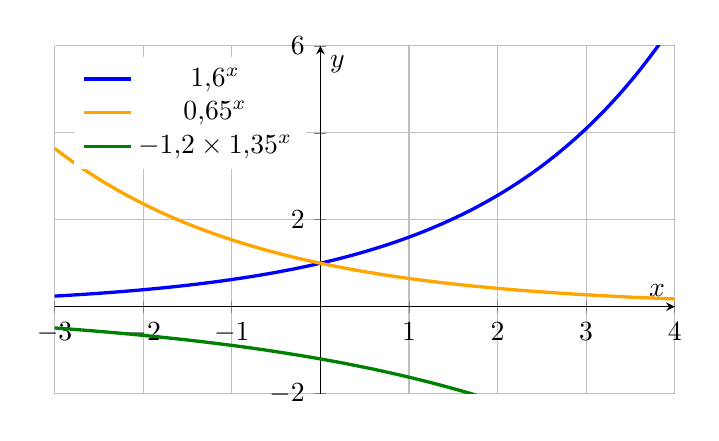
\begin{tikzpicture}
\begin{axis}[width=.78\textwidth,height=6cm,axis lines=middle,xmin=-3,xmax=4,ymin=-2,ymax=6,grid=major,xlabel={$x$},ylabel={$y$},legend style={at={(.03,.97)},anchor=north west,draw=none,fill=white}]
\addplot[Blue,very thick,samples=100,domain=-3:4]{1.6^x};\addlegendentry{$1{,}6^x$}
\addplot[Orange,very thick,samples=100,domain=-3:4]{0.65^x};\addlegendentry{$0{,}65^x$}
\addplot[Green,very thick,samples=100,domain=-3:4]{-1.2*1.35^x};\addlegendentry{$-1{,}2\times1{,}35^x$}
\end{axis}
\end{tikzpicture}
\end{center}

\begin{retenir}
Si $a>1$, $x\mapsto a^x$ est strictement croissante. Si $0<a<1$, elle est strictement décroissante. Pour $f(x)=ka^x$, multiplier par $k<0$ inverse le sens de variation. Dans tous les cas, $a^x>0$.
\end{retenir}

Pour $a>0$ et tous réels $x,y$ :
\[
a^{x+y}=a^xa^y,\qquad a^{x-y}=\frac{a^x}{a^y},\qquad (a^x)^y=a^{xy}.
\]

\begin{erreur}
En général, $a^x+a^y\neq a^{x+y}$. Les propriétés portent sur les produits et les quotients, pas sur les sommes.
\end{erreur}

\subsection{Évolutions et taux moyen}
Une quantité de valeur initiale $V_0$ soumise à une évolution relative constante de coefficient $q$ se modélise par $V(t)=V_0q^t$. Si un coefficient global $Q$ résulte de $n$ évolutions identiques, le coefficient moyen est $q=Q^{\frac1n}$ et le taux moyen est $t=q-1$.

\begin{exemple}
Un chiffre d'affaires passe de $80\,000$ à $95\,000$ euros en quatre ans. Le coefficient global vaut $Q=\dfrac{95\,000}{80\,000}=1{,}1875$. Le coefficient annuel moyen est $q=1{,}1875^{\frac14}\approx1{,}0440$ : le taux annuel moyen est donc environ $4{,}40\,\%$.
\end{exemple}

\subsection{Résoudre et interpréter}
Lorsque les deux membres peuvent être écrits avec la même base, on utilise l'injectivité : pour $a>0$ et $a\neq1$, $a^u=a^v$ équivaut à $u=v$. Sinon, une résolution graphique ou numérique donne une valeur approchée ; le logarithme décimal, étudié ensuite, donnera une formule.

\sessionheader{7}{06/10/2026}{B : 2 h -- C : 1 h}{Définition et sens de variation de $a^x$}{Fonctions exponentielles}
\begin{objectifs}\begin{itemize}\item Donner du sens à $a^x$.\item Relier base et variation.\item Lire des courbes.\end{itemize}\end{objectifs}
\begin{automatismes}\begin{enumerate}\item Écrire le coefficient multiplicateur d'une hausse de $10\,\%$. \rep{$1+\dfrac{10}{100}=1,10$}\item Comparer $1{,}04^3$ et $1{,}04^7$. \rep{$1{,}04^3<1{,}04^7$}\item Calculer $2^4\times2^3$. \rep{$2^7$}\item Écrire $5^{-2}$ sous forme de fraction. \rep{$\dfrac1{25}$}\item La fonction $x\mapsto0{,}7^x$ est-elle croissante ? \rep{Non, elle est décroissante.}\end{enumerate}\end{automatismes}
\begin{prerequis}Relire la dernière trace écrite et savoir effectuer les calculs élémentaires mobilisés aujourd'hui. Avant l'activité, faire reformuler les mots-clés : donner du sens à $a^x$ et relier base et variation.\end{prerequis}

\begin{activite}
À l'aide d'une calculatrice, compléter un tableau de valeurs de $1{,}5^x$ et $0{,}7^x$ pour $x=-2,-1,0,1,2,3$. Tracer les points, conjecturer les variations et identifier le point commun aux deux courbes.
\begin{center}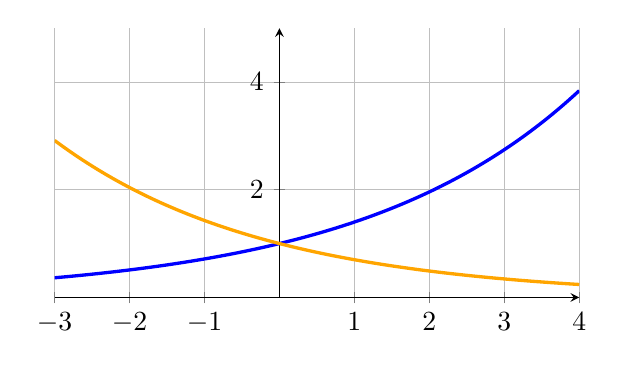
\begin{tikzpicture}\begin{axis}[width=.68\textwidth,height=5cm,axis lines=middle,xmin=-3,xmax=4,ymin=0,ymax=5,grid=major]\addplot[Blue,very thick,samples=100,domain=-3:4]{1.4^x};\addplot[Orange,very thick,samples=100,domain=-3:4]{.7^x};\end{axis}\end{tikzpicture}\end{center}
\end{activite}
\enseignant{$a^0=1$, donc les courbes passent par $(0,1)$. La première croît et la seconde décroît. Faire verbaliser la donnée qui déclenche le choix de méthode.}

\begin{traceecrite}Pour $a>0$, $a^x$ est défini pour tout réel $x$. La fonction est croissante si $a>1$ et décroissante si $0<a<1$.\end{traceecrite}

\begin{exemple}
Reprendre les données de l'activité et rédiger la solution dans l'ordre : définition des objets, propriété utilisée, calcul exact ou approché, puis phrase de réponse. La réponse modèle figure dans l'édition enseignant.
\end{exemple}
\enseignant{$a^0=1$, donc les courbes passent par $(0,1)$. La première croît et la seconde décroît.}

\begin{exercice}[-- essentiel]
\begin{enumerate}\item Simplifier $3^{x+4}\div3^x$ et $(2^x)^3$.\item Étudier le sens de variation de $f(x)=4\times1{,}04^x$ et $g(x)=-4\times0{,}8^x$.\item Une valeur initiale de $1350$ augmente de $4\,\%$ par an. Donner le modèle et calculer la valeur après $6$ ans.\end{enumerate}
\end{exercice}
\enseignant{$3^4$ et $2^{3x}$. $f$ est croissante ; $0{,}8^x$ est décroissante et le coefficient négatif rend $g$ croissante. Le modèle est $V(t)=1350\times\left(1+\dfrac{4}{100}\right)^t$.}

\manuelref{Calao, cours p. 42--47 ; exercices p. 48, n° 1 à 8}
\ExoSession{7}

\begin{dm}Reprendre l'exercice d'entraînement 2 avec les données suivantes : remplacer la donnée initiale par $155$ et le taux ou la raison par $3$. Rédiger en quatre lignes : données, formule, calcul, conclusion.\end{dm}
\enseignant{La correction dépend de l'exercice repris. Vérifier surtout la cohérence du modèle, le nombre d'itérations, l'arrondi et la phrase de conclusion.}

\begin{sortie}Sur une demi-feuille : écrire la règle principale de la séance, traiter un exemple très court et indiquer son degré de confiance de 1 à 4. Question(s) essentielle(s) du jour : 1, 2 et 3.\end{sortie}

\ifprof
\begin{methode}
\textbf{Conduite en 1 h :} 7 min d'automatismes ; 10 min de mise en commun et trace ; 28 min d'exercices essentiels ; 5 min de correction ; 3 min de billet de sortie.\\
\textbf{Conduite en 2 h :} ajouter 20 min de recherche de l'activité, 20 min d'institutionnalisation, un second exercice autonome et 10 min de correction comparée.\\
\textbf{Différenciation :} fournir aux élèves fragiles une fiche à quatre cases (données, modèle, calcul, conclusion). Demander aux élèves rapides de produire un contre-exemple, une justification ou une seconde méthode.
\end{methode}
\fi
\sessionheader{8}{08/10/2026}{B : 1 h -- C : 2 h}{Puissances et propriétés algébriques}{Fonctions exponentielles}
\begin{objectifs}\begin{itemize}\item Transformer des puissances.\item Utiliser les exposants négatifs.\item Repérer une règle inapplicable.\end{itemize}\end{objectifs}
\begin{automatismes}\begin{enumerate}\item Réduire $3x+4-x+2$. \rep{$2x+6$}\item Calculer $2^1\times2^3$. \rep{$2^4$}\item Écrire $5^{-2}$ sous forme de fraction. \rep{$\dfrac1{25}$}\item La fonction $x\mapsto0{,}7^x$ est-elle croissante ? \rep{Non, elle est décroissante.}\item Comparer $1{,}04^3$ et $1{,}04^7$. \rep{$1{,}04^3<1{,}04^7$}\end{enumerate}\end{automatismes}
\begin{prerequis}Relire la dernière trace écrite et savoir effectuer les calculs élémentaires mobilisés aujourd'hui. Avant l'activité, faire reformuler les mots-clés : transformer des puissances et utiliser les exposants négatifs.\end{prerequis}

\begin{activite}
Simplifier $2^3\times2^{-5}$, $5^{x+2}\div5^x$ et $(3^x)^2$. Inventer ensuite un contre-exemple numérique à $a^x+a^y=a^{x+y}$.

\end{activite}
\enseignant{On obtient $2^{-2}=\dfrac14$, $5^2=25$ et $3^{2x}$. Avec $a=2,x=y=1$, $2+2\neq4$ ? Ici égalité accidentelle ; choisir $a=3$ : $3+3\neq9$. Faire verbaliser la donnée qui déclenche le choix de méthode.}

\begin{traceecrite}$a^{x+y}=a^xa^y$, $a^{x-y}=\dfrac{a^x}{a^y}$ et $(a^x)^y=a^{xy}$. Ces règles exigent une même base positive.\end{traceecrite}

\begin{exemple}
Reprendre les données de l'activité et rédiger la solution dans l'ordre : définition des objets, propriété utilisée, calcul exact ou approché, puis phrase de réponse. La réponse modèle figure dans l'édition enseignant.
\end{exemple}
\enseignant{On obtient $2^{-2}=\dfrac14$, $5^2=25$ et $3^{2x}$. Avec $a=2,x=y=1$, $2+2\neq4$ ? Ici égalité accidentelle ; choisir $a=3$ : $3+3\neq9$.}

\begin{exercice}[-- essentiel]
\begin{enumerate}\item Simplifier $3^{x+5}\div3^x$ et $(2^x)^3$.\item Étudier le sens de variation de $f(x)=5\times1{,}05^x$ et $g(x)=-5\times0{,}8^x$.\item Une valeur initiale de $1400$ augmente de $5\,\%$ par an. Donner le modèle et calculer la valeur après $6$ ans.\end{enumerate}
\end{exercice}
\enseignant{$3^5$ et $2^{3x}$. $f$ est croissante ; $0{,}8^x$ est décroissante et le coefficient négatif rend $g$ croissante. Le modèle est $V(t)=1400\times\left(1+\dfrac{5}{100}\right)^t$.}

\manuelref{Calao, cours p. 43--45 ; exercices p. 49, n° 9 à 13}
\ExoSession{8}

\begin{dm}Reprendre l'exercice d'entraînement 3 avec les données suivantes : remplacer la donnée initiale par $160$ et le taux ou la raison par $4$. Rédiger en quatre lignes : données, formule, calcul, conclusion.\end{dm}
\enseignant{La correction dépend de l'exercice repris. Vérifier surtout la cohérence du modèle, le nombre d'itérations, l'arrondi et la phrase de conclusion.}

\begin{sortie}Sur une demi-feuille : écrire la règle principale de la séance, traiter un exemple très court et indiquer son degré de confiance de 1 à 4. Question(s) essentielle(s) du jour : 1 et 2.\end{sortie}

\ifprof
\begin{methode}
\textbf{Conduite en 1 h :} 7 min d'automatismes ; 10 min de mise en commun et trace ; 28 min d'exercices essentiels ; 5 min de correction ; 3 min de billet de sortie.\\
\textbf{Conduite en 2 h :} ajouter 20 min de recherche de l'activité, 20 min d'institutionnalisation, un second exercice autonome et 10 min de correction comparée.\\
\textbf{Différenciation :} fournir aux élèves fragiles une fiche à quatre cases (données, modèle, calcul, conclusion). Demander aux élèves rapides de produire un contre-exemple, une justification ou une seconde méthode.
\end{methode}
\fi
\sessionheader{9}{13/10/2026}{B : 2 h -- C : 1 h}{Fonctions $x\mapsto k a^x$ : variations et graphique}{Fonctions exponentielles}
\begin{objectifs}\begin{itemize}\item Étudier $ka^x$.\item Combiner signe et variation.\item Relier formule et graphique.\end{itemize}\end{objectifs}
\begin{automatismes}\begin{enumerate}\item Calculer $20\,\%$ de $100$. \rep{$20$}\item Écrire $5^{-2}$ sous forme de fraction. \rep{$\dfrac1{25}$}\item La fonction $x\mapsto0{,}7^x$ est-elle croissante ? \rep{Non, elle est décroissante.}\item Comparer $1{,}04^3$ et $1{,}04^7$. \rep{$1{,}04^3<1{,}04^7$}\item Calculer $2^2\times2^3$. \rep{$2^5$}\end{enumerate}\end{automatismes}
\begin{prerequis}Relire la dernière trace écrite et savoir effectuer les calculs élémentaires mobilisés aujourd'hui. Avant l'activité, faire reformuler les mots-clés : étudier $ka^x$ et combiner signe et variation.\end{prerequis}

\begin{activite}
Associer les quatre fonctions $2^x$, $0{,}6^x$, $-2^x$ et $-0{,}6^x$ à quatre courbes. Justifier chaque choix par le signe, le point d'ordonnée à l'origine et le sens de variation.
\begin{center}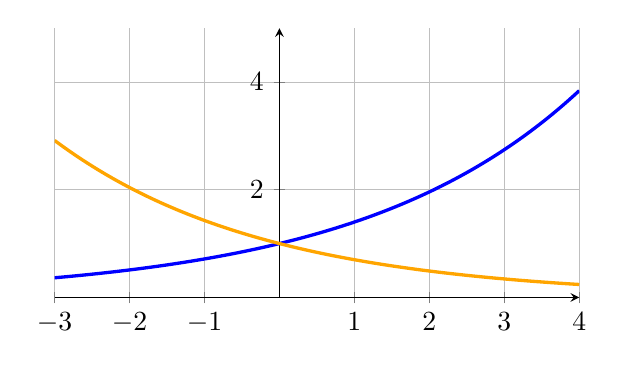
\begin{tikzpicture}\begin{axis}[width=.68\textwidth,height=5cm,axis lines=middle,xmin=-3,xmax=4,ymin=0,ymax=5,grid=major]\addplot[Blue,very thick,samples=100,domain=-3:4]{1.4^x};\addplot[Orange,very thick,samples=100,domain=-3:4]{.7^x};\end{axis}\end{tikzpicture}\end{center}
\end{activite}
\enseignant{Toutes ont une valeur absolue égale à $1$ en $0$. Le signe distingue les deux paires ; la base et le signe du coefficient déterminent la variation. Faire verbaliser la donnée qui déclenche le choix de méthode.}

\begin{traceecrite}Pour $f(x)=ka^x$, le signe est celui de $k$. Si $k<0$, la multiplication par $k$ inverse le sens de variation de $a^x$.\end{traceecrite}

\begin{exemple}
Reprendre les données de l'activité et rédiger la solution dans l'ordre : définition des objets, propriété utilisée, calcul exact ou approché, puis phrase de réponse. La réponse modèle figure dans l'édition enseignant.
\end{exemple}
\enseignant{Toutes ont une valeur absolue égale à $1$ en $0$. Le signe distingue les deux paires ; la base et le signe du coefficient déterminent la variation.}

\begin{exercice}[-- essentiel]
\begin{enumerate}\item Simplifier $3^{x+6}\div3^x$ et $(2^x)^3$.\item Étudier le sens de variation de $f(x)=6\times1{,}06^x$ et $g(x)=-6\times0{,}8^x$.\item Une valeur initiale de $1450$ augmente de $6\,\%$ par an. Donner le modèle et calculer la valeur après $6$ ans.\end{enumerate}
\end{exercice}
\enseignant{$3^6$ et $2^{3x}$. $f$ est croissante ; $0{,}8^x$ est décroissante et le coefficient négatif rend $g$ croissante. Le modèle est $V(t)=1450\times\left(1+\dfrac{6}{100}\right)^t$.}

\manuelref{Calao, cours p. 44--47 ; exercices p. 48, n° 5 à 8, puis p. 52, n° 31 à 36}
\ExoSession{9}

\begin{dm}Reprendre l'exercice d'entraînement 2 avec les données suivantes : remplacer la donnée initiale par $165$ et le taux ou la raison par $5$. Rédiger en quatre lignes : données, formule, calcul, conclusion.\end{dm}
\enseignant{La correction dépend de l'exercice repris. Vérifier surtout la cohérence du modèle, le nombre d'itérations, l'arrondi et la phrase de conclusion.}

\begin{sortie}Sur une demi-feuille : écrire la règle principale de la séance, traiter un exemple très court et indiquer son degré de confiance de 1 à 4. Question(s) essentielle(s) du jour : 1, 2 et 3.\end{sortie}

\ifprof
\begin{methode}
\textbf{Conduite en 1 h :} 7 min d'automatismes ; 10 min de mise en commun et trace ; 28 min d'exercices essentiels ; 5 min de correction ; 3 min de billet de sortie.\\
\textbf{Conduite en 2 h :} ajouter 20 min de recherche de l'activité, 20 min d'institutionnalisation, un second exercice autonome et 10 min de correction comparée.\\
\textbf{Différenciation :} fournir aux élèves fragiles une fiche à quatre cases (données, modèle, calcul, conclusion). Demander aux élèves rapides de produire un contre-exemple, une justification ou une seconde méthode.
\end{methode}
\fi
\sessionheader{10}{15/10/2026}{B : 1 h -- C : 2 h}{Taux d'évolution moyen}{Fonctions exponentielles}
\begin{objectifs}\begin{itemize}\item Calculer un taux moyen.\item Distinguer taux global et moyen.\item Interpréter un exposant $\frac1n$.\end{itemize}\end{objectifs}
\begin{automatismes}\begin{enumerate}\item Écrire le coefficient multiplicateur d'une hausse de $25\,\%$. \rep{$1+\dfrac{25}{100}=1,25$}\item La fonction $x\mapsto0{,}7^x$ est-elle croissante ? \rep{Non, elle est décroissante.}\item Comparer $1{,}04^3$ et $1{,}04^7$. \rep{$1{,}04^3<1{,}04^7$}\item Calculer $2^3\times2^3$. \rep{$2^6$}\item Écrire $5^{-2}$ sous forme de fraction. \rep{$\dfrac1{25}$}\end{enumerate}\end{automatismes}
\begin{prerequis}Relire la dernière trace écrite et savoir effectuer les calculs élémentaires mobilisés aujourd'hui. Avant l'activité, faire reformuler les mots-clés : calculer un taux moyen et distinguer taux global et moyen.\end{prerequis}

\begin{activite}
Le prix d'un service passe de $18$ à $23{,}50$ euros en cinq ans. Calculer le coefficient global, puis le coefficient annuel moyen et le taux annuel moyen. Vérifier en recomposant cinq fois l'évolution.

\end{activite}
\enseignant{$Q=\dfrac{23{,}5}{18}\approx1{,}3056$, $q=Q^{\frac15}\approx1{,}0548$, soit environ $5{,}48\,\%$ par an. Faire verbaliser la donnée qui déclenche le choix de méthode.}

\begin{traceecrite}Si $Q$ est le coefficient global de $n$ évolutions identiques, le coefficient moyen est $q=Q^{\frac1n}$ et le taux moyen est $q-1$.\end{traceecrite}

\begin{exemple}
Reprendre les données de l'activité et rédiger la solution dans l'ordre : définition des objets, propriété utilisée, calcul exact ou approché, puis phrase de réponse. La réponse modèle figure dans l'édition enseignant.
\end{exemple}
\enseignant{$Q=\dfrac{23{,}5}{18}\approx1{,}3056$, $q=Q^{\frac15}\approx1{,}0548$, soit environ $5{,}48\,\%$ par an.}

\begin{exercice}[-- essentiel]
\begin{enumerate}\item Simplifier $3^{x+2}\div3^x$ et $(2^x)^3$.\item Étudier le sens de variation de $f(x)=2\times1{,}02^x$ et $g(x)=-2\times0{,}8^x$.\item Une valeur initiale de $1500$ augmente de $2\,\%$ par an. Donner le modèle et calculer la valeur après $6$ ans.\end{enumerate}
\end{exercice}
\enseignant{$3^2$ et $2^{3x}$. $f$ est croissante ; $0{,}8^x$ est décroissante et le coefficient négatif rend $g$ croissante. Le modèle est $V(t)=1500\times\left(1+\dfrac{2}{100}\right)^t$.}

\manuelref{Calao, cours p. 47--49 ; exercices p. 49, n° 14 à 19, puis p. 54, n° 47 à 50}
\ExoSession{10}

\begin{dm}Reprendre l'exercice d'entraînement 3 avec les données suivantes : remplacer la donnée initiale par $170$ et le taux ou la raison par $6$. Rédiger en quatre lignes : données, formule, calcul, conclusion.\end{dm}
\enseignant{La correction dépend de l'exercice repris. Vérifier surtout la cohérence du modèle, le nombre d'itérations, l'arrondi et la phrase de conclusion.}

\begin{sortie}Sur une demi-feuille : écrire la règle principale de la séance, traiter un exemple très court et indiquer son degré de confiance de 1 à 4. Question(s) essentielle(s) du jour : 1 et 2.\end{sortie}

\ifprof
\begin{methode}
\textbf{Conduite en 1 h :} 7 min d'automatismes ; 10 min de mise en commun et trace ; 28 min d'exercices essentiels ; 5 min de correction ; 3 min de billet de sortie.\\
\textbf{Conduite en 2 h :} ajouter 20 min de recherche de l'activité, 20 min d'institutionnalisation, un second exercice autonome et 10 min de correction comparée.\\
\textbf{Différenciation :} fournir aux élèves fragiles une fiche à quatre cases (données, modèle, calcul, conclusion). Demander aux élèves rapides de produire un contre-exemple, une justification ou une seconde méthode.
\end{methode}
\fi
\sessionheader{11}{03/11/2026}{B : 2 h -- C : 1 h}{Lecture de représentations graphiques}{Fonctions exponentielles}
\begin{objectifs}\begin{itemize}\item Lire images et antécédents.\item Comparer deux modèles.\item Estimer graphiquement.\end{itemize}\end{objectifs}
\begin{automatismes}\begin{enumerate}\item Réduire $3x+7-x+2$. \rep{$2x+9$}\item Comparer $1{,}04^3$ et $1{,}04^7$. \rep{$1{,}04^3<1{,}04^7$}\item Calculer $2^4\times2^3$. \rep{$2^7$}\item Écrire $5^{-2}$ sous forme de fraction. \rep{$\dfrac1{25}$}\item La fonction $x\mapsto0{,}7^x$ est-elle croissante ? \rep{Non, elle est décroissante.}\end{enumerate}\end{automatismes}
\begin{prerequis}Relire la dernière trace écrite et savoir effectuer les calculs élémentaires mobilisés aujourd'hui. Avant l'activité, faire reformuler les mots-clés : lire images et antécédents et comparer deux modèles.\end{prerequis}

\begin{activite}
Deux offres commerciales sont modélisées par $f(x)=120\times1{,}08^x$ et $g(x)=180\times0{,}96^x$. Tracer les courbes sur $[0,12]$, lire leur point d'intersection et interpréter les zones où chaque valeur est la plus grande.
\begin{center}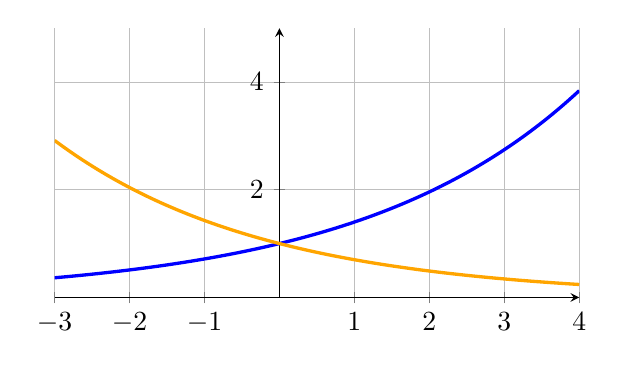
\begin{tikzpicture}\begin{axis}[width=.68\textwidth,height=5cm,axis lines=middle,xmin=-3,xmax=4,ymin=0,ymax=5,grid=major]\addplot[Blue,very thick,samples=100,domain=-3:4]{1.4^x};\addplot[Orange,very thick,samples=100,domain=-3:4]{.7^x};\end{axis}\end{tikzpicture}\end{center}
\end{activite}
\enseignant{La lecture graphique situe l'intersection vers $x\approx3{,}5$. Avant ce rang $g$ domine ; après, $f$ domine. Une valeur approchée est attendue. Faire verbaliser la donnée qui déclenche le choix de méthode.}

\begin{traceecrite}Lire $f(x)$ consiste à partir de $x$ vers la courbe puis vers l'axe des ordonnées. Chercher un antécédent de $y$ consiste à partir de $y$ vers la courbe puis vers l'axe des abscisses.\end{traceecrite}

\begin{exemple}
Reprendre les données de l'activité et rédiger la solution dans l'ordre : définition des objets, propriété utilisée, calcul exact ou approché, puis phrase de réponse. La réponse modèle figure dans l'édition enseignant.
\end{exemple}
\enseignant{La lecture graphique situe l'intersection vers $x\approx3{,}5$. Avant ce rang $g$ domine ; après, $f$ domine. Une valeur approchée est attendue.}

\begin{exercice}[-- essentiel]
\begin{enumerate}\item Simplifier $3^{x+3}\div3^x$ et $(2^x)^3$.\item Étudier le sens de variation de $f(x)=3\times1{,}03^x$ et $g(x)=-3\times0{,}8^x$.\item Une valeur initiale de $1550$ augmente de $3\,\%$ par an. Donner le modèle et calculer la valeur après $6$ ans.\end{enumerate}
\end{exercice}
\enseignant{$3^3$ et $2^{3x}$. $f$ est croissante ; $0{,}8^x$ est décroissante et le coefficient négatif rend $g$ croissante. Le modèle est $V(t)=1550\times\left(1+\dfrac{3}{100}\right)^t$.}

\manuelref{Calao, p. 52, n° 31 à 36}
\ExoSession{11}

\begin{dm}Reprendre l'exercice d'entraînement 2 avec les données suivantes : remplacer la donnée initiale par $175$ et le taux ou la raison par $7$. Rédiger en quatre lignes : données, formule, calcul, conclusion.\end{dm}
\enseignant{La correction dépend de l'exercice repris. Vérifier surtout la cohérence du modèle, le nombre d'itérations, l'arrondi et la phrase de conclusion.}

\begin{sortie}Sur une demi-feuille : écrire la règle principale de la séance, traiter un exemple très court et indiquer son degré de confiance de 1 à 4. Question(s) essentielle(s) du jour : 1, 2 et 3.\end{sortie}

\ifprof
\begin{methode}
\textbf{Conduite en 1 h :} 7 min d'automatismes ; 10 min de mise en commun et trace ; 28 min d'exercices essentiels ; 5 min de correction ; 3 min de billet de sortie.\\
\textbf{Conduite en 2 h :} ajouter 20 min de recherche de l'activité, 20 min d'institutionnalisation, un second exercice autonome et 10 min de correction comparée.\\
\textbf{Différenciation :} fournir aux élèves fragiles une fiche à quatre cases (données, modèle, calcul, conclusion). Demander aux élèves rapides de produire un contre-exemple, une justification ou une seconde méthode.
\end{methode}
\fi
\sessionheader{12}{05/11/2026}{B : 1 h -- C : 2 h}{Équations exponentielles simples}{Fonctions exponentielles}
\begin{objectifs}\begin{itemize}\item Résoudre avec une même base.\item Approcher une solution.\item Vérifier la vraisemblance.\end{itemize}\end{objectifs}
\begin{automatismes}\begin{enumerate}\item Calculer $5\,\%$ de $160$. \rep{$8$}\item Calculer $2^1\times2^3$. \rep{$2^4$}\item Écrire $5^{-2}$ sous forme de fraction. \rep{$\dfrac1{25}$}\item La fonction $x\mapsto0{,}7^x$ est-elle croissante ? \rep{Non, elle est décroissante.}\item Comparer $1{,}04^3$ et $1{,}04^7$. \rep{$1{,}04^3<1{,}04^7$}\end{enumerate}\end{automatismes}
\begin{prerequis}Relire la dernière trace écrite et savoir effectuer les calculs élémentaires mobilisés aujourd'hui. Avant l'activité, faire reformuler les mots-clés : résoudre avec une même base et approcher une solution.\end{prerequis}

\begin{activite}
Résoudre $4^x=64$, $9^x=\dfrac13$ et $1{,}12^x=2$ : d'abord par même base lorsque c'est possible, puis numériquement pour la dernière. Encadrer la dernière solution entre deux entiers.

\end{activite}
\enseignant{$x=3$ ; $9^x=3^{-1}$ donc $2x=-1$ et $x=-\dfrac12$ ; enfin $x\approx6{,}12$, entre $6$ et $7$. Faire verbaliser la donnée qui déclenche le choix de méthode.}

\begin{traceecrite}Pour résoudre $a^x=b$ : utiliser une même base quand c'est possible ; sinon encadrer ou utiliser un outil numérique. Vérifier que $b>0$.\end{traceecrite}

\begin{exemple}
Reprendre les données de l'activité et rédiger la solution dans l'ordre : définition des objets, propriété utilisée, calcul exact ou approché, puis phrase de réponse. La réponse modèle figure dans l'édition enseignant.
\end{exemple}
\enseignant{$x=3$ ; $9^x=3^{-1}$ donc $2x=-1$ et $x=-\dfrac12$ ; enfin $x\approx6{,}12$, entre $6$ et $7$.}

\begin{exercice}[-- essentiel]
\begin{enumerate}\item Simplifier $3^{x+4}\div3^x$ et $(2^x)^3$.\item Étudier le sens de variation de $f(x)=4\times1{,}04^x$ et $g(x)=-4\times0{,}8^x$.\item Une valeur initiale de $1600$ augmente de $4\,\%$ par an. Donner le modèle et calculer la valeur après $6$ ans.\end{enumerate}
\end{exercice}
\enseignant{$3^4$ et $2^{3x}$. $f$ est croissante ; $0{,}8^x$ est décroissante et le coefficient négatif rend $g$ croissante. Le modèle est $V(t)=1600\times\left(1+\dfrac{4}{100}\right)^t$.}

\manuelref{Calao, p. 52, n° 37--38, puis p. 54, n° 45--46}
\ExoSession{12}

\begin{dm}Reprendre l'exercice d'entraînement 3 avec les données suivantes : remplacer la donnée initiale par $180$ et le taux ou la raison par $2$. Rédiger en quatre lignes : données, formule, calcul, conclusion.\end{dm}
\enseignant{La correction dépend de l'exercice repris. Vérifier surtout la cohérence du modèle, le nombre d'itérations, l'arrondi et la phrase de conclusion.}

\begin{sortie}Sur une demi-feuille : écrire la règle principale de la séance, traiter un exemple très court et indiquer son degré de confiance de 1 à 4. Question(s) essentielle(s) du jour : 1 et 2.\end{sortie}

\ifprof
\begin{methode}
\textbf{Conduite en 1 h :} 7 min d'automatismes ; 10 min de mise en commun et trace ; 28 min d'exercices essentiels ; 5 min de correction ; 3 min de billet de sortie.\\
\textbf{Conduite en 2 h :} ajouter 20 min de recherche de l'activité, 20 min d'institutionnalisation, un second exercice autonome et 10 min de correction comparée.\\
\textbf{Différenciation :} fournir aux élèves fragiles une fiche à quatre cases (données, modèle, calcul, conclusion). Demander aux élèves rapides de produire un contre-exemple, une justification ou une seconde méthode.
\end{methode}
\fi
\sessionheader{13}{10/11/2026}{B : 2 h -- C : 1 h}{Modélisation par une fonction exponentielle}{Fonctions exponentielles}
\begin{objectifs}\begin{itemize}\item Construire un modèle exponentiel.\item Identifier les paramètres.\item Prévoir et interpréter.\end{itemize}\end{objectifs}
\begin{automatismes}\begin{enumerate}\item Écrire le coefficient multiplicateur d'une hausse de $10\,\%$. \rep{$1+\dfrac{10}{100}=1,10$}\item Écrire $5^{-2}$ sous forme de fraction. \rep{$\dfrac1{25}$}\item La fonction $x\mapsto0{,}7^x$ est-elle croissante ? \rep{Non, elle est décroissante.}\item Comparer $1{,}04^3$ et $1{,}04^7$. \rep{$1{,}04^3<1{,}04^7$}\item Calculer $2^2\times2^3$. \rep{$2^5$}\end{enumerate}\end{automatismes}
\begin{prerequis}Relire la dernière trace écrite et savoir effectuer les calculs élémentaires mobilisés aujourd'hui. Avant l'activité, faire reformuler les mots-clés : construire un modèle exponentiel et identifier les paramètres.\end{prerequis}

\begin{activite}
Une application compte $12\,000$ utilisateurs au lancement et sa fréquentation augmente de $9\,\%$ par mois. Construire $f(t)$, calculer $f(6)$, puis déterminer numériquement quand elle dépassera $25\,000$ utilisateurs.
\begin{center}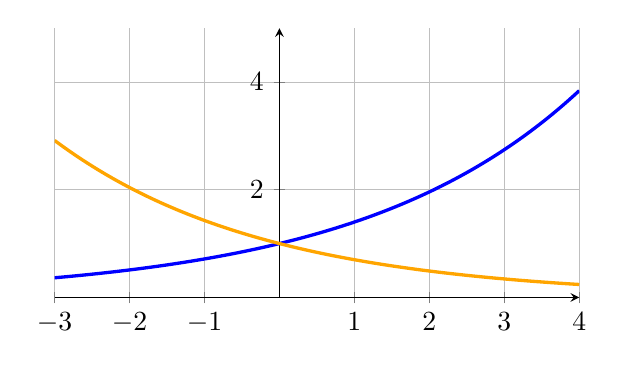
\begin{tikzpicture}\begin{axis}[width=.68\textwidth,height=5cm,axis lines=middle,xmin=-3,xmax=4,ymin=0,ymax=5,grid=major]\addplot[Blue,very thick,samples=100,domain=-3:4]{1.4^x};\addplot[Orange,very thick,samples=100,domain=-3:4]{.7^x};\end{axis}\end{tikzpicture}\end{center}
\end{activite}
\enseignant{$f(t)=12\,000\times1{,}09^t$, $f(6)\approx20\,126$. Le seuil est dépassé à partir du neuvième mois. Faire verbaliser la donnée qui déclenche le choix de méthode.}

\begin{traceecrite}Une évolution relative constante de coefficient $q$ se modélise par $f(t)=V_0q^t$. $V_0$ est la valeur initiale et $q$ le coefficient par unité de temps.\end{traceecrite}

\begin{exemple}
Reprendre les données de l'activité et rédiger la solution dans l'ordre : définition des objets, propriété utilisée, calcul exact ou approché, puis phrase de réponse. La réponse modèle figure dans l'édition enseignant.
\end{exemple}
\enseignant{$f(t)=12\,000\times1{,}09^t$, $f(6)\approx20\,126$. Le seuil est dépassé à partir du neuvième mois.}

\begin{exercice}[-- essentiel]
\begin{enumerate}\item Simplifier $3^{x+5}\div3^x$ et $(2^x)^3$.\item Étudier le sens de variation de $f(x)=5\times1{,}05^x$ et $g(x)=-5\times0{,}8^x$.\item Une valeur initiale de $1650$ augmente de $5\,\%$ par an. Donner le modèle et calculer la valeur après $6$ ans.\end{enumerate}
\end{exercice}
\enseignant{$3^5$ et $2^{3x}$. $f$ est croissante ; $0{,}8^x$ est décroissante et le coefficient négatif rend $g$ croissante. Le modèle est $V(t)=1650\times\left(1+\dfrac{5}{100}\right)^t$.}

\manuelref{Calao, p. 50, n° 20 à 25, puis p. 53, n° 41}
\ExoSession{13}

\begin{dm}Reprendre l'exercice d'entraînement 2 avec les données suivantes : remplacer la donnée initiale par $185$ et le taux ou la raison par $3$. Rédiger en quatre lignes : données, formule, calcul, conclusion.\end{dm}
\enseignant{La correction dépend de l'exercice repris. Vérifier surtout la cohérence du modèle, le nombre d'itérations, l'arrondi et la phrase de conclusion.}

\begin{sortie}Sur une demi-feuille : écrire la règle principale de la séance, traiter un exemple très court et indiquer son degré de confiance de 1 à 4. Question(s) essentielle(s) du jour : 1, 2 et 3.\end{sortie}

\ifprof
\begin{methode}
\textbf{Conduite en 1 h :} 7 min d'automatismes ; 10 min de mise en commun et trace ; 28 min d'exercices essentiels ; 5 min de correction ; 3 min de billet de sortie.\\
\textbf{Conduite en 2 h :} ajouter 20 min de recherche de l'activité, 20 min d'institutionnalisation, un second exercice autonome et 10 min de correction comparée.\\
\textbf{Différenciation :} fournir aux élèves fragiles une fiche à quatre cases (données, modèle, calcul, conclusion). Demander aux élèves rapides de produire un contre-exemple, une justification ou une seconde méthode.
\end{methode}
\fi
\sessionheader{14}{12/11/2026}{B : 1 h -- C : 2 h}{Bilan et évaluation du chapitre}{Fonctions exponentielles}
\begin{objectifs}\begin{itemize}\item Mobiliser les acquis du chapitre.\item Rédiger une modélisation.\item Corriger une erreur.\end{itemize}\end{objectifs}
\begin{automatismes}\begin{enumerate}\item Réduire $3x+3-x+2$. \rep{$2x+5$}\item La fonction $x\mapsto0{,}7^x$ est-elle croissante ? \rep{Non, elle est décroissante.}\item Comparer $1{,}04^3$ et $1{,}04^7$. \rep{$1{,}04^3<1{,}04^7$}\item Calculer $2^4\times2^3$. \rep{$2^7$}\item Écrire $5^{-2}$ sous forme de fraction. \rep{$\dfrac1{25}$}\end{enumerate}\end{automatismes}
\begin{prerequis}Relire la dernière trace écrite et savoir effectuer les calculs élémentaires mobilisés aujourd'hui. Avant l'activité, faire reformuler les mots-clés : mobiliser les acquis du chapitre et rédiger une modélisation.\end{prerequis}

\begin{activite}
À partir de quatre productions d'élèves, repérer et corriger : confusion taux/coefficient, propriété de puissances fausse, erreur de sens de variation et conclusion sans unité.

\end{activite}
\enseignant{La correction doit nommer l'erreur, écrire la règle correcte, reprendre le calcul et conclure dans le contexte. Faire verbaliser la donnée qui déclenche le choix de méthode.}

\begin{traceecrite}Pour valider un modèle exponentiel : identifier $V_0$ et $q$, calculer avec les unités, vérifier l'ordre de grandeur et interpréter le résultat.\end{traceecrite}

\begin{exemple}
Reprendre les données de l'activité et rédiger la solution dans l'ordre : définition des objets, propriété utilisée, calcul exact ou approché, puis phrase de réponse. La réponse modèle figure dans l'édition enseignant.
\end{exemple}
\enseignant{La correction doit nommer l'erreur, écrire la règle correcte, reprendre le calcul et conclure dans le contexte.}

\begin{exercice}[-- essentiel]
\begin{enumerate}\item Simplifier $3^{x+6}\div3^x$ et $(2^x)^3$.\item Étudier le sens de variation de $f(x)=6\times1{,}06^x$ et $g(x)=-6\times0{,}8^x$.\item Une valeur initiale de $1700$ augmente de $6\,\%$ par an. Donner le modèle et calculer la valeur après $6$ ans.\end{enumerate}
\end{exercice}
\enseignant{$3^6$ et $2^{3x}$. $f$ est croissante ; $0{,}8^x$ est décroissante et le coefficient négatif rend $g$ croissante. Le modèle est $V(t)=1700\times\left(1+\dfrac{6}{100}\right)^t$.}

\manuelref{Calao, p. 54, n° 47 à 58}
\ExoSession{14}

\begin{dm}Reprendre l'exercice d'entraînement 3 avec les données suivantes : remplacer la donnée initiale par $190$ et le taux ou la raison par $4$. Rédiger en quatre lignes : données, formule, calcul, conclusion.\end{dm}
\enseignant{La correction dépend de l'exercice repris. Vérifier surtout la cohérence du modèle, le nombre d'itérations, l'arrondi et la phrase de conclusion.}

\begin{sortie}Sur une demi-feuille : écrire la règle principale de la séance, traiter un exemple très court et indiquer son degré de confiance de 1 à 4. Question(s) essentielle(s) du jour : 1 et 2.\end{sortie}

\ifprof
\begin{methode}
\textbf{Conduite en 1 h :} 7 min d'automatismes ; 10 min de mise en commun et trace ; 28 min d'exercices essentiels ; 5 min de correction ; 3 min de billet de sortie.\\
\textbf{Conduite en 2 h :} ajouter 20 min de recherche de l'activité, 20 min d'institutionnalisation, un second exercice autonome et 10 min de correction comparée.\\
\textbf{Différenciation :} fournir aux élèves fragiles une fiche à quatre cases (données, modèle, calcul, conclusion). Demander aux élèves rapides de produire un contre-exemple, une justification ou une seconde méthode.
\end{methode}
\fi
